\section{Lektion 30-01-2018}

\begin{enumerate}
	\item Course introduction
	\item Typical embedded system
	\item Number formats (fixed- and floating-point)
	\item Conversion between different number formats
	\item (Blackfin) DSP Architecture
	\item Software development flow
\end{enumerate}

\begin{mdframed}[style=exampledefault]
\begin{itemize}
	\item ESP Chapter 1.1 + 1.2
	\item ESP 5.1 + 5.2.1
	\item ESP Chapter 6.1.1 (only p.217-p.222) and 6.1.3 - 6.1.5
\end{itemize}
\end{mdframed}

\subsection{Typical embedded system}

\begin{itemize}
	\item \textbf{Dedicated functions:} Embedded systems usaully execute a specific task repeatedly. 
	\item \textbf{Tight constraints:} There are many constraints in designing an embedded system, such as; cost, processing speed, size, power consuption. 
	\item \textbf{Reactive and real-time performance:} Many embedded systems must continously react to changes of the system's input.
\end{itemize}

\subsection{Number formats (fixed- and floating-point)}
\begin{itemize}
	\item Fixed‐point
	\item Floating‐point
	\item Block floating‐point
\end{itemize}

\subsubsection{Fixed-point}

\begin{itemize}
	\item  Binary data format - signed and unsigned
	\begin{itemize}
		\item  The 2's complement format is	the most popular signed number in DSP processors.
		\item Most DSP processors support both integer and fractional data formats.
		\begin{itemize}
			\item  In an integer format, the radix point is located to the right of the least
			significant bit (LSB).
			\item In a fractional number format, the radix point is located within the binary number. 
			\begin{itemize}
				\item The number to the right	of the radix point assumes a fractional binary bit, with a weighting of $2^{-p}$ where the lowest fractional increment is $2^{−4}$ (or $0.0625$) in \ref{fig:1}.
				\item For the number to the left of the radix point, the weighting increases from $2^q$. The weighting of the MSB (or sign bit) depends on whether the number is signed or unsigned. 
			\end{itemize}
			\item (N.M) notation
			\begin{itemize}
				\item  N is the number of bits to the left of the radix point (integer part).
				\item M is the number of bits to the right of the radix point (fractional part). 
				\item The symbol \textit{"."} represents the radix point. 
				\item Total number of bits in the data word is B = N + M. 
			\end{itemize}
		\end{itemize}
	\end{itemize}
\end{itemize}

\begin{figure} [H]
	\centering
	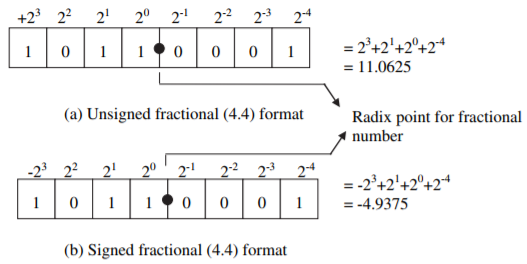
\includegraphics[width=0.85\linewidth]{graphics/1.png}
	\caption{Example of 8-bit binary data formats for a fractional number.}
	\label{fig:1}
\end{figure}

\begin{itemize}
	\item Dynamic Ranges and Precisions
	\begin{itemize}
		\item The maximum positive number in (1.15) format is $1 − 2^{−15} (= 0.999969482421875)$ (0x7FFF).
		\item The minimum negative number in (1.15) format is $−1$ (0x8000). 
		\item The 1.15 format has a \textbf{dynamic range} of $[+0.999969482421875$ to $−1]$
		\begin{itemize}
			\item Numbers exceeding this range cannot be represented in 1.15 format. 
		\end{itemize} 
		\item The smallest increment (or precision) within the (1.15) format is $2^{−15}$.
	\end{itemize}
	\item Scaling Factors
	\begin{itemize}
		\item A number in (N.M) format cannot be represented in the programs because most compilers and assemblers only recognize numbers in integer or (16.0) format. 
		\begin{itemize}
			\item Convert the fractional number in (N.M) format into its integer equivalent.
			\item Its radix point must be accounted for by the programmers.
			\begin{itemize}
				\item To convert a number $0.6$ in (1.15) format to its integer representation,
				multiply it by $2^{15}$ (or $32\,768$) and round the product to its nearest integer to
				become $19\,661$ (0x4CCD).
			\end{itemize}
		\end{itemize}
	\end{itemize}
\end{itemize}

 In table \ref{fig:2} all 16 possible (N.M) formats for 16-bit numbers. Different formats give different dynamic ranges and precisions. There is a trade-off between the dynamic range and precision.
 \begin{itemize}
 	\item As the dynamic range increases, precision becomes	coarser.
 \end{itemize}
 
\begin{figure} [H]
 	\centering
 	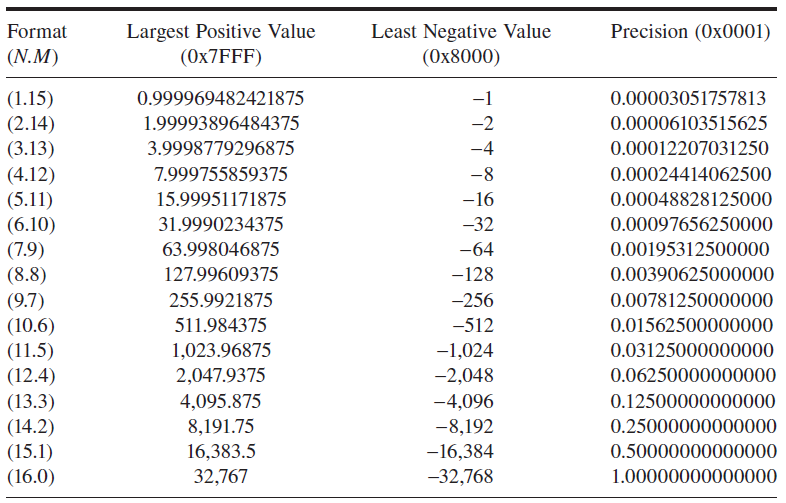
\includegraphics[width=\linewidth]{graphics/2.png}
 	\caption{Dynamic ranges and precisions of 16-bit numbers using different formats.}
 	\label{fig:2}
\end{figure}

\begin{figure} [H]
	\centering
	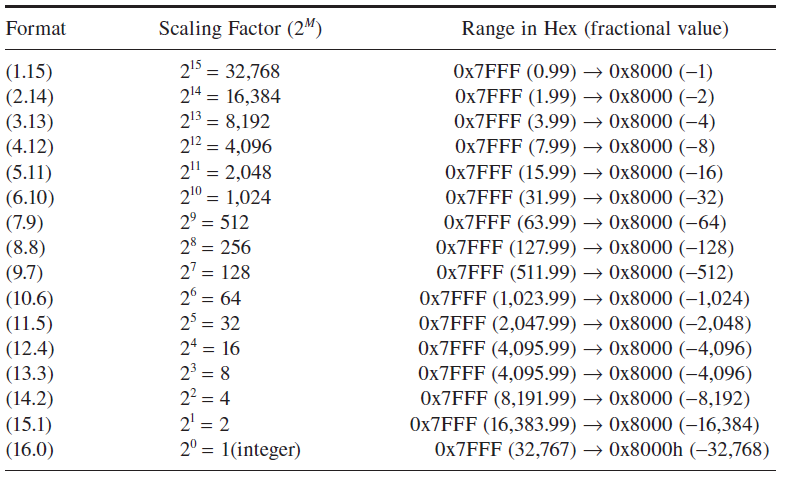
\includegraphics[width=\linewidth]{graphics/8.png}
	\caption{Scaling factors and dynamic ranges for 16-bit numbers using different formats.}
	\label{fig:8}
\end{figure}

\subsection{Conversion between different number formats}
\subsubsection{Fixed-Point Data Types}
The Blackfin C compiler supports eight scalar data types and two fractional data types.

\begin{figure} [H]
	\centering
	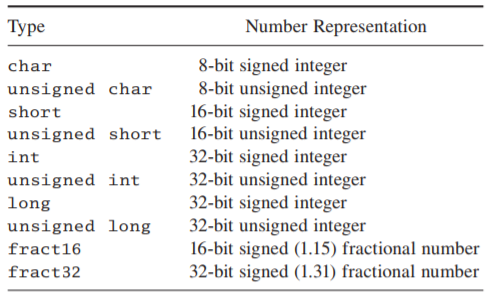
\includegraphics[width=0.85\linewidth]{graphics/3.png}
	\caption{Fixed-Point Data Types.}
	\label{fig:3}
\end{figure}

\subsection{(Blackfin) DSP Architecture}
The Von Neumann architecture uses a single memory to hold both data and instructions. In comparison, the Harvard architecture uses separate memories 
for data and instructions, providing higher speed. The Super Harvard Architecture improves upon Harvard design by adding an instruction cache and a dedicated I/O controller. 

\subsubsection{Von Neumann Architecture}
\begin{figure} [H]
	\centering
	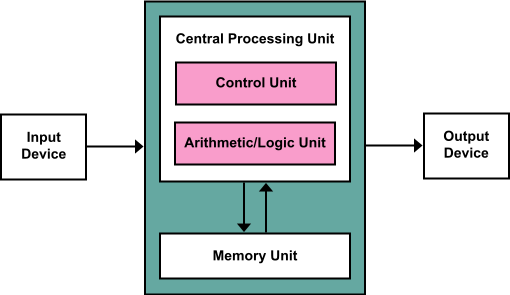
\includegraphics[width=0.85\linewidth]{graphics/4.png}
	\caption{Von Neumann Architecture (single memory).}
	\label{fig:4}
\end{figure}

\subsubsection{Super Harvard Architecture}
\begin{figure} [H]
	\centering
	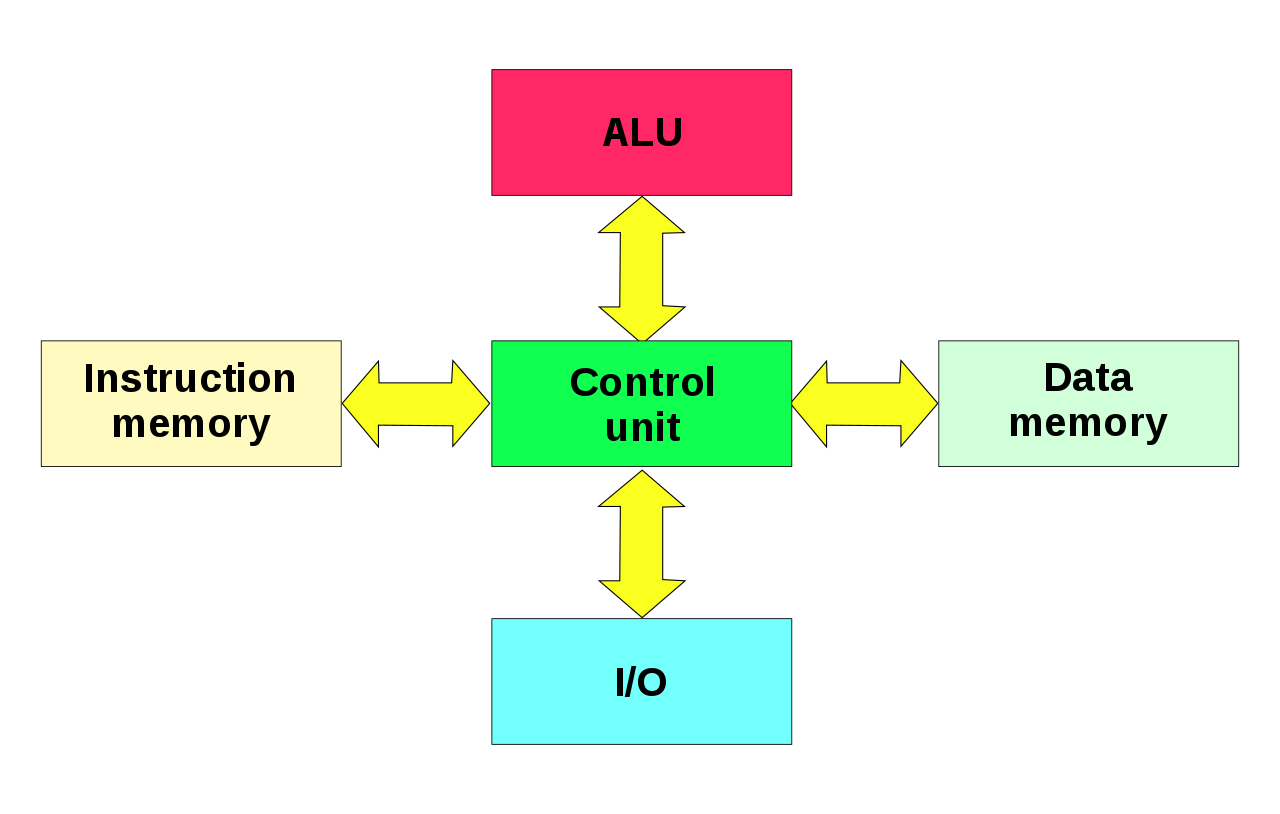
\includegraphics[width=0.85\linewidth]{graphics/5.png}
	\caption{Super Harvard Achitecture (dual memory, instruction cache, I/O controller)}
	\label{fig:5}
\end{figure}

\subsection{Choice of processor}
\begin{itemize}
	\item DSP
	\begin{itemize}
		\item Harvard memory architecture (optimized for the operational needs of digital signal processing).
		\item Handle real time processing, architecture is specially designed to fetch multiple data at the same time.
		\item Can handle floating numbers directly in the data flow path.
		\item Calculations are usually carried out by fixed point arithmetic process in order to speed them up.
	\end{itemize}
	\item Microcontroller
	\item General‐purpose CPU
	\begin{itemize}
		\item Most general-purpose CPU can also execute DSP algorithms successfully, but dedicated DSPs usually have better power efficiency.
	\end{itemize}
	\item FPGA
	\item GPU
\end{itemize}

\subsection{Blackfin}
\begin{itemize}
	\item Blackfin is a \textit{MSA} Processor.
	\begin{itemize}
		\item MCU and DSP in same processor.
		\begin{itemize}
			\item Cheap and low power consumption.
		\end{itemize}
	\end{itemize}
	\item Architecture optimized for multimedia	processing (Audio and Video).
	\item Dataflow oriented tasks (DSP).
	\item Control flow oriented tasks (MCU).
	\item Good tools and compiler support.
\end{itemize}

\subsubsection{BF533 Overview}
\begin{figure} [H]
	\centering
	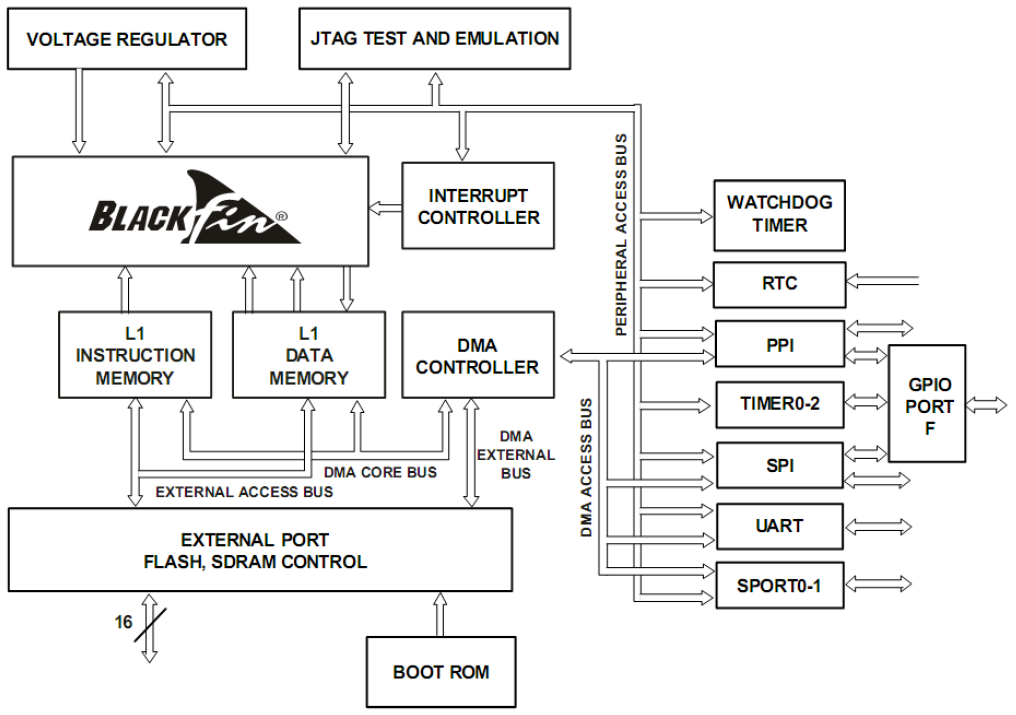
\includegraphics[width=0.85\linewidth]{graphics/6.png}
	\caption{BF533 Overview.}
	\label{fig:6}
\end{figure}

\subsubsection{Blackfin Core}

\begin{figure} [H]
	\centering
	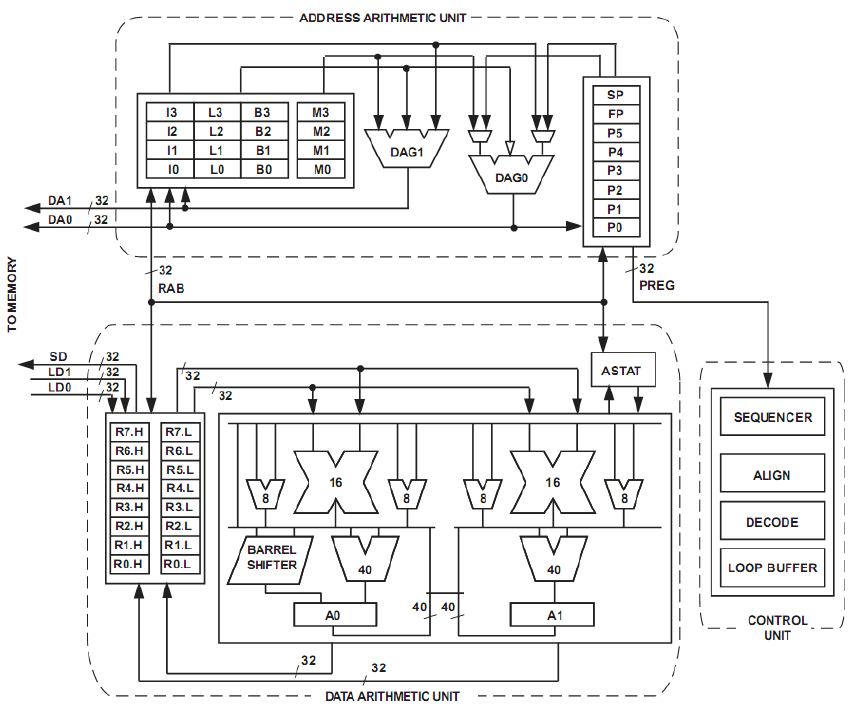
\includegraphics[width=0.85\linewidth]{graphics/7.png}
	\caption{BF533 Core, Fixed-point processor.}
	\label{fig:7}
\end{figure}
